\documentclass[conference]{IEEEtran}
\usepackage[T1]{fontenc}\usepackage[utf8]{inputenc}
\usepackage{amsmath,graphicx,booktabs,cite}
\begin{document}
\title{ESGenius: Evidence-Grounded, Human-in-the-Loop Gap Analysis of SEBI BRSR Disclosures Using Lexical Retrieval and Batched LLM Classification}
\author{\IEEEauthorblockN{Aditya Sinha}\IEEEauthorblockA{Department of Computer Engineering\\Vidyalankar Institute of Technology, Wadala, Mumbai, India} \and \IEEEauthorblockN{Sehaj Alag}\IEEEauthorblockA{Department of Computer Engineering\\Vidyalankar Institute of Technology, Wadala, Mumbai, India} \and \IEEEauthorblockN{Pradnesh Jadhav}\IEEEauthorblockA{Department of Computer Engineering\\Vidyalankar Institute of Technology, Wadala, Mumbai, India} \and \IEEEauthorblockN{Gaurav Deore}\IEEEauthorblockA{Department of Computer Engineering\\Vidyalankar Institute of Technology, Wadala, Mumbai, India}}
\maketitle
\begin{abstract}Listed Indian companies must file a Business Responsibility and Sustainability Report (BRSR) that answers 140 disclosure questions defined by the Securities and Exchange Board of India (SEBI). Checking a draft report against every question is slow, manual and error-prone. This paper presents ESGenius, a web-based decision-support system that ingests a sustainability PDF, retrieves page-cited evidence for each BRSR question and classifies each question as covered, partially covered, not covered or requiring human review. Evidence selection is deterministic: page-bounded chunking is followed by a BM25-style lexical scorer extended with ESG term aliases, phrase anchors and a discriminative-term gate. A large language model (Google Gemini) is used only for classification, and requirements are batched by BRSR section so that a full 140-question analysis needs 15 model calls instead of 140. Deterministic fallbacks prevent the model from inventing coverage: no retrieved evidence yields \textit{not covered} without a model call, and any model failure yields \textit{human review required}. On the Infosys BRSR for FY 2024-25 (49 pages), the retriever returned evidence for all 140 questions; an audit judged the top-ranked passage relevant for 119 (85.0\%) and at least partially relevant for 129 (92.1\%) of them. Errors concentrate in short identity fields of Section A and in the tabular layout of Section B. The system is a prototype that supports, and does not replace, professional judgement.\end{abstract}
\begin{IEEEkeywords}ESG reporting, SEBI BRSR, retrieval-augmented generation, BM25, large language models, compliance gap analysis, document understanding\end{IEEEkeywords}
\section{Introduction}
Environmental, social and governance (ESG) disclosure has moved from voluntary reporting to a regulatory obligation. In India, SEBI requires the top listed entities to publish a Business Responsibility and Sustainability Report (BRSR) as part of their annual report \cite{b1}. The BRSR format contains 140 numbered questions: general disclosures (Section A), management and process disclosures (Section B) and, for each of the nine principles of the National Guidelines on Responsible Business Conduct, \textit{Essential} and \textit{Leadership} indicators (Section C).

Before filing, a sustainability team must check that a draft report answers every question and that each answer is supported by data. This is a reading task over documents that routinely exceed 100 pages and mix prose with multi-column tables. The work is repetitive, depends on individual reviewers, and gaps are often found late. Large language models (LLMs) can read and summarise such documents, but applying them naively to compliance work is risky: a model may assert that a disclosure exists when it does not, and its answers are hard to trace to a source page \cite{b10}.

This paper describes ESGenius, a prototype that treats the model as one component in a controlled pipeline rather than as the decision maker. Its contributions are:

(1) A \textbf{page-aware ingestion and retrieval pipeline} that attaches every piece of evidence to a PDF page number and selects it without a model, using a BM25-style lexical scorer \cite{b2} with ESG term aliases, phrase anchors and gating rules.

(2) \textbf{Section-batched LLM classification} that reduces a full 140-question analysis from 140 model calls to 15, which makes a complete analysis feasible within a 20-requests-per-day free-tier quota.

(3) A \textbf{fail-safe decision policy}: absence of evidence is classified deterministically as not covered, and any model failure degrades to \textit{human review required} instead of a guess.

(4) An \textbf{end-to-end implementation} with authentication, per-user document ownership, usage limits, asynchronous processing, progress reporting and a PDF gap-assessment export, together with a retrieval audit on a real BRSR.

The remainder of the paper is organised as follows. Section II reviews related work, Section III presents the architecture, Section IV details the method, Section V summarises the implementation and testing, Section VI reports the evaluation, and Sections VII and VIII discuss limitations and conclude.

\section{Background and Related Work}
\subsection{The BRSR Framework}
The BRSR was introduced by SEBI circular SEBI/HO/CFD/CMD-2/P/CIR/2021/562 of 10 May 2021 \cite{b1}. ESGenius encodes the 140 questions of the original Annexure I format as framework requirements and stores, for each, a code, title, description, section, indicator type and framework text. Table I shows the composition of the requirement set. Later revisions of the format (BRSR Core, value-chain and assurance requirements) are outside the present scope.

\begin{table}[!t]\centering\caption{BRSR Requirement Set and Batch Plan (L = 12)}
\footnotesize\begin{tabular}{lcccc}\toprule
Section & Gen./Ess. & Lead. & Total & Calls \\ \midrule
A (General) & 24 & - & 24 & 2 \\
B (Management) & 12 & - & 12 & 1 \\
P1 & 7 & 2 & 9 & 1 \\
P2 & 4 & 5 & 9 & 1 \\
P3 & 15 & 6 & 21 & 2 \\
P4 & 2 & 3 & 5 & 1 \\
P5 & 10 & 5 & 15 & 2 \\
P6 & 12 & 9 & 21 & 2 \\
P7 & 2 & 1 & 3 & 1 \\
P8 & 4 & 6 & 10 & 1 \\
P9 & 6 & 5 & 11 & 1 \\
Total & 98 & 42 & 140 & 15 \\
\bottomrule\end{tabular}
\end{table}
\subsection{NLP for Corporate Sustainability Reports}
Domain-adapted language models such as ClimateBERT \cite{b6} and datasets such as ClimaText \cite{b7} target climate-related text classification, for example detecting whether a sentence concerns climate risk. ChatReport \cite{b5} uses an LLM to answer questions about sustainability reports and makes answers traceable to source passages, motivated by the hallucination problem. ESGenius differs in its target and its control flow: it maps a document to a fixed, legally defined question set, produces a status for each question, and restricts what the model is allowed to decide.

\subsection{Retrieval-Augmented Generation}
Retrieval-augmented generation (RAG) grounds a generator in retrieved passages \cite{b3}, \cite{b4}. Dense retrieval is common, but lexical BM25 \cite{b2} remains a strong zero-shot baseline across heterogeneous collections \cite{b8}. Regulatory questionnaires are phrased in stable, domain-specific vocabulary, and a lexical retriever is cheap, needs no embedding service, is deterministic and its scores can be inspected. ESGenius therefore uses lexical retrieval and reserves the LLM for the judgement step. Long prompts can also degrade a model's use of information placed in the middle of the context \cite{b9}; this motivates keeping retrieved evidence short and capping the batch size.

\section{System Architecture}
ESGenius is a three-tier web application. The frontend is a React 19 application built with TanStack Start, Router and Query on Vite and TypeScript. The backend is a Java 21 / Spring Boot 3.4 service exposing a versioned REST API. Data are stored in PostgreSQL, with the schema managed by 12 Flyway migrations (12 tables) and validated against the JPA entities at start-up. Uploaded PDFs are kept on the server file system; metadata, per-page text and analysis results are kept in the database.

\textit{Authentication and access control.} Users sign in with Supabase Auth. The frontend sends the access token as a bearer token, and a servlet filter validates it against Supabase and caches successful validations keyed by a SHA-256 digest of the token. Every document is owned by the uploading user; seeded sample documents have no owner and are view-only except for administrators. Requests for another user's private document return 404.

\textit{Asynchronous processing.} Upload returns immediately with status PROCESSING while a bounded background executor extracts text (Apache PDFBox \cite{b12}, without OCR) and stores it page by page. A compliance analysis likewise runs on its own executor and the UI polls its status. Documents or analyses left in progress by a restart are marked FAILED at start-up so that no job stays pending forever.

\textit{Resource protection.} Uploads are limited to 25 MB, 400 pages and three million extracted characters. Rolling per-user caps apply to uploads (20 per day), analyses (5 per day) and assistant questions (30 per hour), and a global cap of 20 analyses per day protects the shared model quota; over-limit calls return HTTP 429 with a Retry-After header.

\begin{figure}[!t]\centering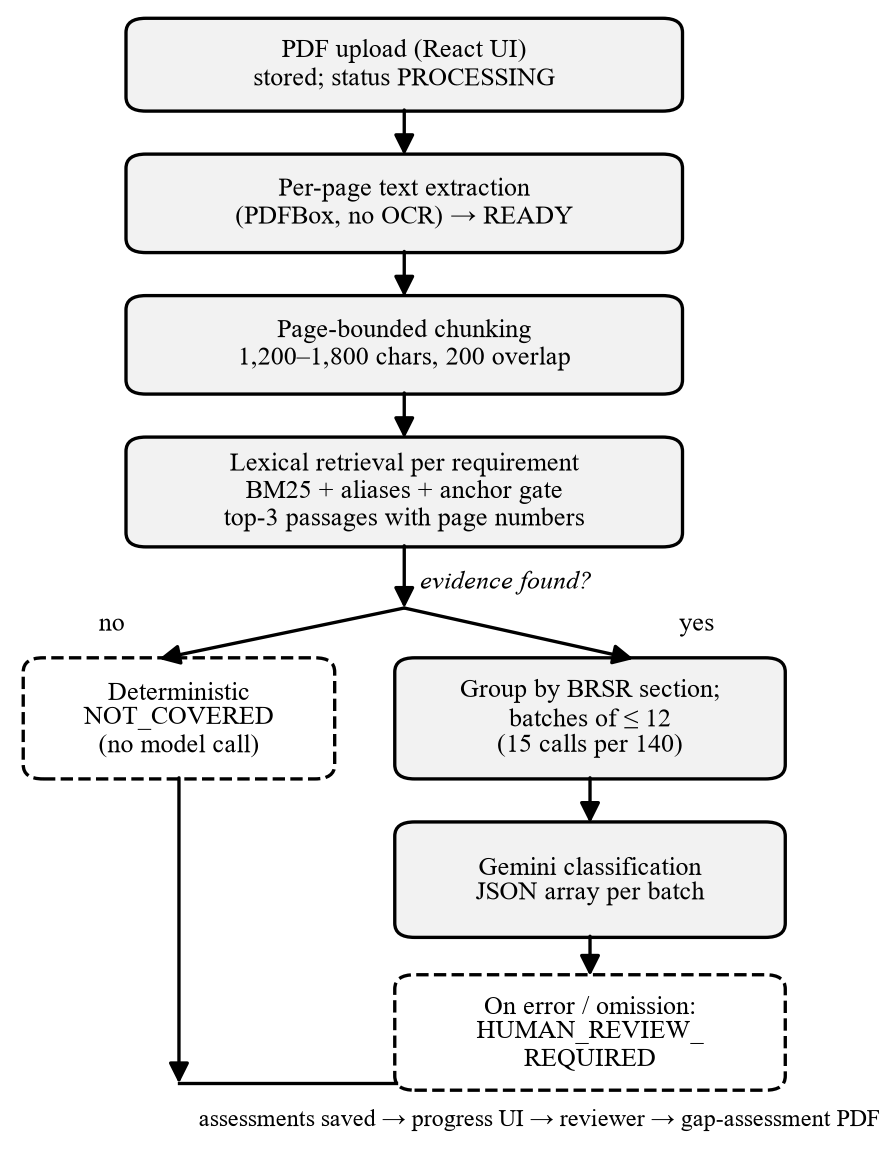
\includegraphics[width=0.95\columnwidth]{fig1_pipeline.png}
\caption{ESGenius analysis pipeline. Dashed boxes are deterministic fail-safe paths.}\end{figure}
\section{Method}
\subsection{Page-Aware Chunking}
Extracted text is kept per page. Each page is split into chunks of about 1,200-1,800 characters, breaking preferably at a newline, full stop or semicolon, with a 200-character overlap. Chunks never cross a page boundary, so every retrieved passage carries an exact 1-based page number that is later shown to the reviewer and printed in the report.

\subsection{Lexical Evidence Retrieval}
For each requirement, a weighted query is built from its code (weight 3.0), title (6.0) and description (2.5). Stop-words and a list of generic BRSR words (for example \textit{entity}, \textit{report}, \textit{policy}) are removed, and curated ESG aliases are added at 0.85 of the weight of their seed term, for example \textit{bribery} for \textit{corruption} or \textit{kilolitres} for \textit{water}. Each chunk is split into sentence-level passages, and each passage \textit{p} is scored against every query term \textit{t} with a BM25 term score:

\begin{equation}s(t,p)=w_t\,\mathrm{idf}(t)\,\frac{\mathrm{tf}_{t,p}(k_1+1)}{\mathrm{tf}_{t,p}+k_1\left(1-b+b\,\frac{|p|}{\bar L}\right)}\end{equation}
where \textit{w\_t} is the field weight of the term, \textit{tf} the term frequency in the passage, |\textit{p}| the passage length in tokens and \textit{$\bar{L}$} the mean chunk length of the document. The constants are \textit{k\_1} = 1.2 and \textit{b} = 0.75, and the inverse document frequency is computed over the chunks of the uploaded document:

\begin{equation}\mathrm{idf}(t)=\max\!\left(\ln\!\left(\frac{N-\mathrm{df}_t+0.5}{\mathrm{df}_t+0.5}+1\right),\,0.05\right)\end{equation}
with \textit{N} the number of chunks; for generic terms the raw value is first multiplied by 0.05. Because the unit of scoring is a passage inside a chunk, the best-matching sentence is returned rather than a whole chunk. The passage score adds bonuses for phrase-level evidence:

\begin{equation}S(p)=\max\!\Big(0,\ \sum_t s(t,p)+5A(p)+4L(p)+8R(p)+10C(p)-40F(p)\Big)\end{equation}
where \textit{A} counts matched title/description phrase anchors, \textit{L} matched alias phrases, \textit{R} is 1 if a required-anchor phrase occurs (stop-words may be inserted between its tokens, so \textit{waste recycled} matches \textit{waste was recycled}), \textit{C} is 1 if the Scope number in the requirement title occurs in the passage, and \textit{F} counts forbidden phrases. A passage that names a different GHG Scope than the requirement is rejected outright, which separates the Scope 1, 2 and 3 questions.

A passage is eligible only if it passes an \textit{anchor gate}: it must match a required anchor if the requirement defines one; otherwise it must contain an anchor or alias phrase or at least two non-generic discriminative query terms. This gate removes passages that score well only because of common words. The three highest-scoring chunks whose best passage scores at least 0.15 are returned together with their page numbers. If none qualifies, the requirement has no evidence. Curated required-anchor and forbidden-phrase lists exist for the original 14 prototype requirements; the audit in Section VI exercises the generic path used for all 140 questions.

\subsection{Evidence Preparation}
A matched passage is often a sentence fragment, so before classification it is expanded inside its chunk by 350 characters before and 550 characters after the match, capped at 1,800 characters. This gives the model local context, such as a table heading, without sending the whole page.

\subsection{Section-Batched Classification}
Requirements that have evidence are classified by Google Gemini \cite{b11} into one of four statuses: COVERED, PARTIALLY\_COVERED, NOT\_COVERED or HUMAN\_REVIEW\_REQUIRED, each with a confidence, an explanation, a gap and a recommendation. The prompt fixes the model's role: the requirement title, description and framework text are declared the \textit{complete} rubric; the model must not import criteria from outside knowledge of BRSR, SEBI or other standards, must not judge whether a metric is good or bad, and must not claim certification.

A one-request-per-question design would need 140 calls per analysis. Because the free-tier quota of the model used was 20 requests per day, requirements are grouped by BRSR section (A, B, P1-P9) and each group is split as evenly as possible into the fewest batches of at most \textit{L} = 12 requirements. For a group of \textit{n} requirements, the number of batches is \textit{m} = $\lceil$\textit{n}/\textit{L}$\rceil$ and the batch sizes are $\lfloor$\textit{n}/\textit{m}$\rfloor$ or $\lfloor$\textit{n}/\textit{m}$\rfloor$+1. Each prompt lists, for every requirement, its own rubric and its own evidence passages, instructs the model to evaluate each independently, and asks for a JSON array keyed by the requirement code. Grouping by section keeps related questions together and the per-call context short. For the full BRSR set this yields 15 calls (Table I).

\begin{table}[!t]\centering\caption{Model Calls per Full Analysis (140 Requirements)}
\footnotesize\begin{tabular}{lcc}\toprule
Strategy & Calls & Fits 20/day? \\ \midrule
One call per requirement & 140 & No \\
Section batches, L = 12 & 15 & Yes (5 spare) \\
\bottomrule\end{tabular}
\end{table}
\subsection{Fail-Safe Decision Policy}
The model never creates coverage on its own. (i) A requirement without retrieved evidence is classified NOT\_COVERED by a deterministic classifier with confidence 0.75 and no model call. (ii) If the model omits a requirement or returns an invalid entry, only that requirement falls back to HUMAN\_REVIEW\_REQUIRED. (iii) If a call fails, all requirements of that batch fall back to HUMAN\_REVIEW\_REQUIRED. (iv) Retryable errors are retried with exponential backoff, honouring a server-supplied retry delay; once the daily quota is exhausted, remaining calls are skipped and the explanation shown to the user states the quota reason. The result is a conservative asymmetry: errors push work to a human instead of producing a false COVERED.

\section{Implementation and Testing}
Besides gap analysis, the system provides a document-grounded assistant that answers questions about one uploaded document: it retrieves passages with the same lexical retriever, cites them, and, when nothing matches, returns a fixed not-found answer with the flag grounded = false without calling the model. Completed analyses can be exported as a Gap Assessment PDF that embeds page citations and a disclaimer that the output is prototype decision support requiring human validation. A company-comparison view shows seeded, illustrative ESG scores; these are not model outputs and are labelled as prototype data.

The repository records 90 commits between 14 August and 20 October 2026. At the time of writing it contains 370 backend JUnit test methods and 124 frontend Vitest cases. Backend tests run against an in-memory H2 database in PostgreSQL mode with the same Flyway scripts; the live model and live authentication are replaced by in-process fakes or mocked HTTP servers, so tests never call external services. Dedicated tests cover batch planning (limit respected for every limit/size combination, 140 requirements giving 15 calls), prompt construction, parsing of partial or malformed model answers, quota handling, asynchronous job recovery, ownership rules and rate limiting.

\section{Evaluation}
\subsection{Setup}
We evaluated the retrieval stage on the Infosys Limited BRSR for the financial year April 2024 - March 2025, a 49-page publicly available report that produced 92 chunks. All 140 active requirements were run through the production retriever; no model was called. For each requirement the top-ranked passage was graded against the requirement title: \textit{relevant} (the passage is the disclosure or its table or question text), \textit{partially relevant} (a related but different disclosure) or \textit{not relevant}. The grading measures topical relevance of the top result (precision at 1), not whether the disclosed value is correct, and a per-requirement listing is provided as supplementary material.

\subsection{Retrieval Results}
The retriever returned at least one passage for all 140 requirements (140 of 140). Table III and Fig. 2 give the audit outcome. The top passage was relevant for 119 requirements (85.0\%) and at least partially relevant for 129 (92.1\%). Performance was high for the nine principles of Section C (96 of 104 relevant, 92.3\%), where questions are long and descriptive, and in every case for Principles 1-4 and 7-8. It was lowest in Section B (5 of 12, 41.7\%) and Section A (18 of 24, 75.0\%).

\begin{table}[!t]\centering\caption{Top-1 Retrieval Audit on the Infosys BRSR FY 2024-25}
\footnotesize\begin{tabular}{lccccc}\toprule
Group & n & Rel. & Part. & Not & P@1 \\ \midrule
Section A & 24 & 18 & 2 & 4 & 75.0\% \\
Section B & 12 & 5 & 4 & 3 & 41.7\% \\
Principles 1-9 & 104 & 96 & 4 & 4 & 92.3\% \\
All & 140 & 119 & 10 & 11 & 85.0\% \\
\bottomrule\end{tabular}
\par\vspace{2pt}{\scriptsize\textit{P@1: share of requirements whose top passage is relevant (strict).}}
\end{table}
\textit{Error analysis.} The 11 non-relevant results fall into three groups. First, four short identity fields in Section A (corporate address, e-mail, website, paid-up capital) returned generic header or contact lines such as \textit{Name of the Listed Entity}. Second, several questions share vocabulary and compete for the same passage: four Principle 5 questions (human-rights complaints, assessments of plants, value-chain assessments and corrective action) all returned the identical \textit{scope and coverage of human rights due diligence} passage with the same score (103.9). Third, three Section B questions (value-chain extension of policies, targets, reasons for uncovered principles) returned text from other sections. We did not analyse causes in depth; a plausible factor for Section B is that its answers are given in a multi-column table that a line-based text extractor flattens, which is consistent with the limitations of lexical, line-based retrieval discussed in Section VII.

\subsection{Model-Call Budget}
Table II compares call budgets. Without batching, a full analysis needs one call per requirement with evidence, up to 140, which cannot complete under a 20-request daily quota. Section batching needs 15 calls, leaving five requests for retries and other use. The first prototype, with 14 requirements, used 14 calls per analysis and already consumed most of the daily quota; extending to the full set therefore required batching.

\subsection{Threats to Validity}
The retrieval audit uses a single report from one large IT company that follows the BRSR format closely, so results may not transfer to reports with different layouts or to scanned documents. Grading was done by a single rater, an AI assistant, whose labels were not verified by human raters, so no inter-rater agreement is available. Because the report discloses nearly every item, the evidence-absent path (deterministic NOT\_COVERED) was not exercised on real data. Finally, the quality of the LLM classification itself (agreement with expert labels) has not yet been measured; this requires an expert-labelled corpus and live model quota and is the main item of future work.

\section{Limitations and Future Work}
\textit{Scope.} Only the original BRSR Annexure I format is supported; BRSR Core, value-chain and assurance disclosures are not. Other frameworks (GRI, IFRS S1/S2, ESRS) are planned only. \textit{Retrieval.} Lexical, line-based retrieval is weak on multi-column tables and on short factual fields; table-aware extraction and hybrid lexical-dense retrieval are natural next steps. \textit{Documents.} There is no OCR, so scanned PDFs are rejected. \textit{Batching.} Requirements in a batch share one call, so one failed call affects up to 12 requirements, and an answer cannot use another requirement's evidence by design. \textit{Operations.} Rate limits are held in memory per instance and the file store is local, which limits horizontal scaling. \textit{Evaluation.} We plan an expert-labelled benchmark of several BRSR reports to measure classification accuracy, calibration of the confidence value and the reduction in reviewer time.

\textit{Responsible use.} ESGenius classifies disclosure coverage, not ESG performance, and does not certify compliance. Outputs are intended to prioritise a human reviewer's attention; the interface, the exported PDF and the model prompt all state this.

\section{Conclusion}
We presented ESGenius, a pipeline that checks a sustainability report against the 140 questions of the SEBI BRSR with page-cited evidence. Combining deterministic lexical retrieval, section-batched LLM classification and conservative fallbacks lets the system run a complete analysis in 15 model calls while ensuring that missing evidence and model failures never produce a claim of compliance. An audit on a real BRSR found the top-ranked evidence relevant for 85.0\% of questions, with identifiable weaknesses in identity fields and tables. Future work will measure classification quality against expert labels and add table-aware and hybrid retrieval.

\section*{Acknowledgment}The authors thank their project mentor, Dr. Amit Aylani, for his guidance during the project.
\begin{thebibliography}{99}
\bibitem{b1} Securities and Exchange Board of India, "Business responsibility and sustainability reporting by listed entities," Circular SEBI/HO/CFD/CMD-2/P/CIR/2021/562, May 10, 2021.
\bibitem{b2} S. Robertson and H. Zaragoza, "The probabilistic relevance framework: BM25 and beyond," \textit{Found. Trends Inf. Retr.}, vol. 3, no. 4, pp. 333-389, 2009.
\bibitem{b3} P. Lewis \textit{et al.}, "Retrieval-augmented generation for knowledge-intensive NLP tasks," in \textit{Proc. Adv. Neural Inf. Process. Syst. (NeurIPS)}, vol. 33, 2020, pp. 9459-9474.
\bibitem{b4} Y. Gao \textit{et al.}, "Retrieval-augmented generation for large language models: A survey," arXiv:2312.10997, 2023.
\bibitem{b5} J. Ni \textit{et al.}, "ChatReport: Democratizing sustainability disclosure analysis through LLM-based tools," in \textit{Proc. EMNLP 2023 System Demonstrations}, Singapore, Dec. 2023, pp. 21-51, doi: 10.18653/v1/2023.emnlp-demo.3.
\bibitem{b6} N. Webersinke, M. Kraus, J. A. Bingler, and M. Leippold, "ClimateBERT: A pretrained language model for climate-related text," arXiv:2110.12010, 2021.
\bibitem{b7} F. S. Varini, J. Boyd-Graber, M. Ciaramita, and M. Leippold, "ClimaText: A dataset for climate change topic detection," arXiv:2012.00483, 2020.
\bibitem{b8} N. Thakur, N. Reimers, A. Ruckl\'e, A. Srivastava, and I. Gurevych, "BEIR: A heterogeneous benchmark for zero-shot evaluation of information retrieval models," in \textit{Proc. NeurIPS Datasets and Benchmarks Track}, 2021.
\bibitem{b9} N. F. Liu \textit{et al.}, "Lost in the middle: How language models use long contexts," \textit{Trans. Assoc. Comput. Linguistics}, vol. 12, pp. 157-173, 2024.
\bibitem{b10} Z. Ji \textit{et al.}, "Survey of hallucination in natural language generation," \textit{ACM Comput. Surv.}, vol. 55, no. 12, Art. no. 248, 2023.
\bibitem{b11} Gemini Team, Google, "Gemini: A family of highly capable multimodal models," arXiv:2312.11805, 2023.
\bibitem{b12} Apache Software Foundation, "Apache PDFBox." [Online]. Available: https://pdfbox.apache.org
\end{thebibliography}
\end{document}